\section{Esquema físic de configuració}


\subsection{Racks}

Els racks es composen de màquines que subministren el mateix servei, és a dir, màquines amb el mateix rol dins del conjunt de l'aplicació. Es procedeix amb aquesta organització per tal de disposar d'homogenització a l'hora de provisionar l'ample de banda que ha de disposar cada rack. Tots els racks són de 42Us.

Cada rack disposarà de dos switchos de "top-of-rack", a més dels nodes pertinents. 

A continuació s'especifiquen els racks que cal provisionar de cada perfil. 

\begin{description}

\item[Comunicacions] \hfill \\ 
    Hi haurà un rack de comunicacions de xarxa amb quatre switchos. Dos seran els de "core-front" i els altres dos seran de "core-backend". Els dos "core-front" disposaran d'un mòdul de routing que donarà sortida cap a internet. Cada mòdul tindrà dos enllaços agregats cap a internet. 
    
\item[LoadBalancers] \hfill \\
    Hi haurà dos racks de LoadBalancers amb trenta màquines cadascun.

\item[Frontals] \hfill \\
    Hi haurà quatre-cents nodes allotjats en onze racks i cada rack disposarà de 39 nodes. Un d'ells disposarà de 28Us lliures per provisionar màquines de tipus "Frontal".

\item[Aplicació] \hfill \\
    Hi haurà vint nodes allotjats en un rack. 
    
\item[Emmagatzematge] \hfill \\
    Hi haurà un racka d'emmagatzematge. El qual disposarà de sis clústers de storage. Aquests es composen de dos nodes NFS i d'una cabina de discs (JBOD).

\begin{figure}[H]
    \centering
    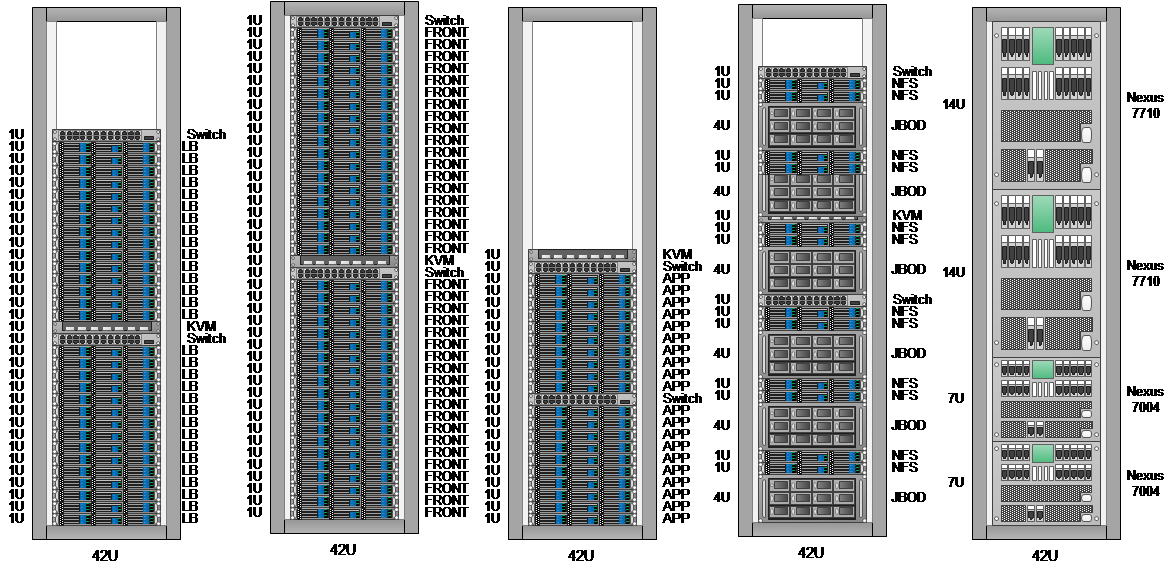
\includegraphics[width=1.0\textwidth]{racks}
    \caption{Definició de racks \label{fig:racks}}    
\end{figure}


\end{description}

\subsection{Enllaços de Xarxa}
\label{sec:links-xarxa}
A continuació es defineixen els amples de banda que hi haurà entre les capes de l'aplicació.

    \begin{description}
    
        \item[Xarxa Externa] \hfill \\
            La sortida a internet serà de 400Gbps. Caldran dos routers per poder agregar el tràfic. Cadascun podrà subministrar dos enllaços de 100Gbps. 
            
            El "oversubscription rate" és de \textbf{1:1}.
        
        \item[LoadBalancers] \hfill \\
            L'enllaç entre els racks de LoadBalancers i els switchos de "core-front" serà de 400Gbps. Caldran 10 enllaços de 40Gbps QSFP+. Els nodes es conectaran mitjançant un enllaç 10Gb Ethernet als switchos de "top-of-rack". Cal tenir en compte que hi haurà dos racks, per tant, els 400Gbps es dividiran en 200Gbps per rack. 

El "oversubscription rate" és 300/200 = 1.5 $\rightarrow$ \textbf{1.5:1}. En conseqüència cada node podrà subministrar 200/300 = 0.66 $\rightarrow$ 0.66*10Gb = 6.66Gbps de pujada com a màxim.
            
        
        \item[Frontals-frontend] \hfill \\
            La conexió entre cadascun dels racks de frontals i els dos switchos de core serà a 39Gbps. L'ample de banda s'aconsegueix amb un enllaç QSFP+ redundat a 40Gbps, per cada rack. Cada node del rack disposarà d'un enllaç de 1Gb Ethernet, el qual podrà subministrar en la seva totalitat. 

El "oversubscription rate" és 39/40 = 0.975 $\rightarrow$ \textbf{0.975:1}. 
        
        \item[Frontals-backend] \hfill \\
           La conexió entre cadascun dels racks de frontals i els switchos de "core-backend" serà de 8Gbps. Tot i que els enllaços seran de 10Gb Ethernet. L'ample de banda disponible equival al percentatge de "miss" de les caches de frontals, un 20\%. Inicialment aquest percentatge és més elevat, no obstant, s'assumeix un període de "warm-up".
           
            El "oversubscription rate" es calcula a partir del 20\% de l'ample de banda dels frontals i el nombre de racks. Per tant, (40Gbps * 0.2) * 11 racks = 88Gbps. Donat que hi ha quatre enllaços agregats entre el switch de "core-backend" i el rack d'emmagatzematge, el "oversubscription rate" és 88/40 = 2.2 $\rightarrow$ \textbf{2.2:1}.
            
            
        \item[Aplicació] \hfill \\
           L'enllaç dels nodes d'aplicació serà 20Gbps, composats per dos links de 10Gb Ethernet. Els nodes disposaran d'un enllaç de 1Gb Ethernet. 
        
           El "oversubscription rate" és 200/200 = 1 (20 nodes a 1Gbps/ 20Gbps) $\rightarrow$ \textbf{1:1}
           
        \item[Emmagatzematge] \hfill \\
            El rack estarà enllaçat per quatre links de 10Gb Ethernet. Per tant, una velocitat agregada de 40Gbps. Cada node de NFS disposarà d'un link de 10Gb, no obstant, la velocitat dels discs SAS és de 6Gbps. Per tant, hi ha un coll d'ampolla en els discs. Cada cabina JBOD exportarà els volums al clúster de NFS respectiu mitjançant un enllaç SCSI.  
        
            Donat que hi ha 6 clústers d'emmagatzematge, el tràfic agregat serà de 6*6 = 36Gbps. Per tant, el "oversubscription rate" és 36/40 = 0.9 $\rightarrow$ \textbf{0.9:1}
            
            
         \item[Enllaç de Backups] \hfill \\
            Hi haurà un enllaç entre els switchos de "core-backend" a 20Gbps per conectar amb el rack d'emmagatzematge de backup.
            
    \end{description}



\subsection{Arquitectura de Xarxa}

La xarxa es composarà de switchos de "top-of-rack" i de switchos de "core". Hi haurà dos switchos de 48 ports Gigabit ethernet per cada rack. Tot i que un switch sigui suficient per conectar tots els nodes, es provisionen dos per garantir l'alta disponibilitat. Les màquines es conectaran amb una interfície de xarxa a un dels switchos del rack i amb una segona interfície de xarxa al switch del rack adjacent, entre racks del mateix rol. El switchos "top-of-rack" estaran conectats a un switch de core. 

Hi haurà quatre switchos de "core": "core-frontend" i "core-backend", emparellats de dos en dos. Una parella conectarà els racks de frontals amb els racks de LoadBalancers i aquests amb el router que dóna sortida a internet. La segona parella formarà el backbone de l'aplicació. Donaran enllaç entre els servidors d'emmagatezmatge, els d'aplicacions i els frontals. També disposaran de conectivitat amb el centre de dades de backup per facilitar la replicació de les cabines de disc. 

\begin{figure}[H]
    \centering
    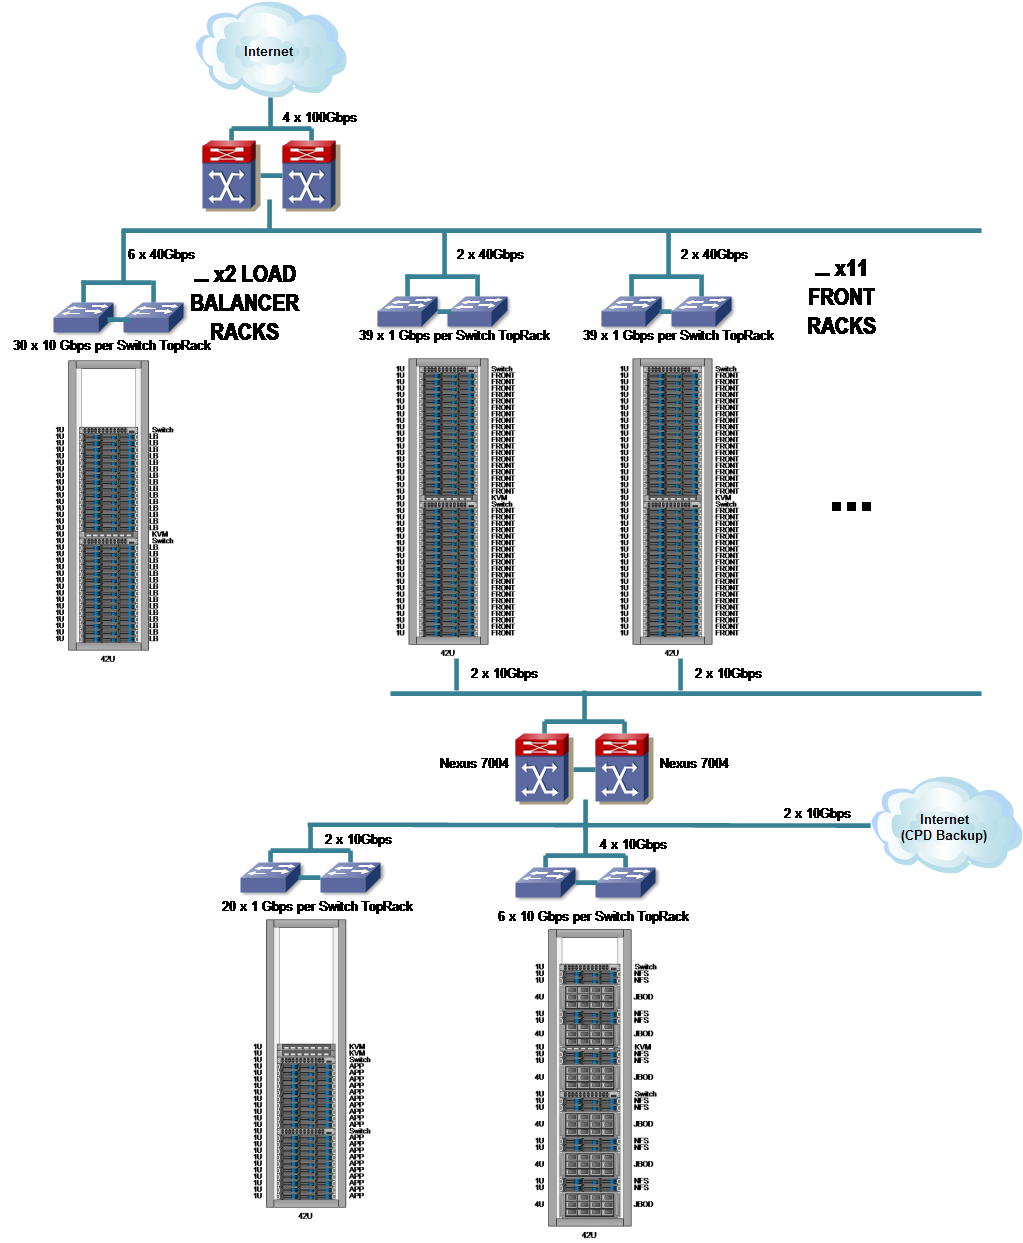
\includegraphics[width=0.85 \textwidth]{cpdnetwork}
    \caption{Arquitectura de Xarxa \label{fig:cpd}}    
\end{figure}

\subsection{Descripció de màquines}

Segons les necessitats descrites anteriorment a l’arquitectura del sistema, proposem el següent maquinari ajustat a les característiques tècniques de hardware requerides. D’una banda es descriurà el hardware dels nodes que aprovisionen el servei i de l’altra es descriuran els models i les funcionalitats dels dispositius de xarxa.

\subsubsection{Nodes}

Proposem 5 tipus de nodes diferents: Front, LoadBalancer, App, NFS i la cabina de discos (o JBOD) amb les següents prestacions:

\begin{description}
    \item[Front - Servidor Frontal Web] \hfill \\
        \vspace{-5mm}
        \begin{itemize}[leftmargin=*]
            \item CPU: Xeon Processor E5-2697 - 12 Nuclis a 2,7GHz
            \\\url{http://ark.intel.com/es-es/products/75283/Intel-Xeon-Processor-E5-2697-v2-30M-Cache-2\_70-GHz}
            \item Memòria: 4 Mòduls de 8GB a 1600Mhz DDR3
            \item Disc: 4TB SATA a 6Gb/s funciona a 7200RPM
            \item Xarxa: 2 Interficies 1GbE amb connexió RJ45
            \item Chasis: Ocupa 1U i NO disposa de font redundant (350W)
        \end{itemize}
    
    \item[LoadBalancer - Servidor Balancejador de Càrrega] \hfill \\
        \vspace{-5mm}
        \begin{itemize}[leftmargin=*]
            \item CPU: Xeon Processor E5-2650 - 8 Nuclis a 2,6GHz 
            \\\url{http://ark.intel.com/es-es/products/64590/Intel-Xeon-Processor-E5-2650-20M-Cache-2\_00-GHz-8\_00-GTs-Intel-QPI}
            \item Memòria: 8 Mòduls de 8GB a 1600Mhz DDR3
            \item Disc: 500GB SATA a 6Gb/s funciona a 7200RPM
            \item Xarxa: 2 Interficies 10GbE amb connexió RJ45
            \item Chasis: Ocupa 1U i disposa de font redundant (700W)
        \end{itemize}
        
    \item[App - Servidor d'Aplicació] \hfill \\
        \vspace{-5mm}
        \begin{itemize}[leftmargin=*]
            \item CPU: Xeon Processor E3-1220L - 2 Nuclis a 2,2GHz 
            \\\url{http://ark.intel.com/es-es/products/53401/Intel-Xeon-Processor-E3-1220L-3M-Cache-2\_20-GHz}
            \item Memòria: 2 Mòduls de 8GB a 1600Mhz DDR3
            \item Disc: 500GB SATA a 6Gb/s funciona a 7200RPM
            \item Xarxa: 2 Interficies 1GbE amb connexió RJ45
            \item Chasis: Ocupa 1U i NO disposa de font redundant (200W)
        \end{itemize}
        
    \item[NFS - Servidor de NFS] \hfill \\
        \vspace{-5mm}
        \begin{itemize}[leftmargin=*]
            \item CPU: Xeon Processor E5-2650 - 8 Nuclis a 2,6GHz 
            \\\url{http://ark.intel.com/es-es/products/64590/Intel-Xeon-Processor-E5-2650-20M-Cache-2\_00-GHz-8\_00-GTs-Intel-QPI}
            \item Memòria: 8 Mòduls de 16GB a 1600Mhz DDR3
            \item Disc: 500GB SATA a 6Gb/s funciona a 7200RPM
            \item Xarxa: 2 Interficies 10GbE amb connexió RJ45
            \item Controladora RAID: MegaRAID SAS 9286CV-8e - 8 Ports a 6b/s amb  1GB SDRAM
            \\\url{http://www.lsi.com/products/raid-controllers/pages/megaraid-sas-9286cv-8e.aspx}
            \item Chasis: Ocupa 1U i disposa de font redundant (700W)
        \end{itemize}
        
    \item[JBOD - Caixa de discos] \hfill \\
        \vspace{-5mm}
        \begin{itemize}[leftmargin=*]
            \item Disc: 90 unitats de 4TB SATA a 6Gb/s funciona a 7200RPM
            \\\url{http://www.seagate.com/www-content/product-content/enterprise-hdd-fam/enterprise-capacity-3-5-hdd/constellation-es-4/es-es/docs/enterprise-capacity-3-5-hdd-ds1791-3-1403es.pdf}
            \item Chasis: Ocupa 4U i disposa de font redundada (2000W)
        \end{itemize}
    
    
\end{description}

\subsubsection{Dispositius de xarxa}

Proposem 3 tipus de switchos diferents segons la seva situació, de major a menor prestacions són els següents:

\begin{description}
    \item[Switch Front Core] \hfill \\
        \vspace{-5mm}
        \begin{itemize}[leftmargin=*]
            \item Model: Cisco Nexus 7710 (10 Slots, 8 disponibles per IO) 
            \\\url{http://www.cisco.com/c/en/us/products/switches/nexus-7700-10-slot-switch/index.html}
            \item Slots: 1 x 12 Ports 100GbE (CPAK), 2 x 24 Ports 40GbE (QSPF+) 
            \item Chasis: Ocupa 14U i disposa de fonts redundants (9000W)
        \end{itemize}
        
    \item[Switch Bottom Core] \hfill \\
        \vspace{-5mm}
        \begin{itemize}[leftmargin=*]
            \item Model: Cisco Nexus 7004 (4 Slots, 2 disponibles per IO) 
            \\\url{http://www.cisco.com/c/en/us/products/switches/nexus-7000-4-slot-switch/index.html}
            \item Slots: 1 x 48 Ports 10GbE (RJ45), 1 x 24 Ports 10GbE (SPF+) 
            \item Chasis: Ocupa 7U i disposa de fonts redundants (6000W)
        \end{itemize}
        
    \item[Switch Top of Rack] \hfill \\
        \vspace{-5mm}
        \begin{itemize}[leftmargin=*]
            \item Model: Cisco Nexus 3064-T
            \\\url{http://www.cisco.com/c/en/us/products/collateral/switches/nexus-3000-series-switches/data\_sheet\_c78-651097.html}
            \item Slot: 48 Ports 10GbE (RJ45) + 4 Ports 10GbE (QSPF+) 
            \item Chasis: Ocupa 1U i no disposa de font redundant (362W)
        \end{itemize}

\end{description}

\subsection{Arquitectura del sistema d’emmagatzematge}
\label{sec:arquitectura-emmagatzematge}

La infraestructura que es provisiona en el projecte està pensada per facilitar al client provinent d'internet dades estàtiques. Per tant, l'emmagatzematge i l'accés a les dades és un punt molt rellevant en el projecte. 

L'arquitectura del sistema d'emmagatzematge consta, principalment, de tres parts. En primer lloc, hi ha les cabines de discs durs (JBOD). En segon lloc, hi ha els clústers de servidors de NFS i en tercer lloc hi ha els discs dels nodes Frontals.

Hi ha sis cabines de discs durs. Cadascuna està composada de 90 discs de 4TB SATA amb una velocitat de rotació de 7200rpm. Això significa que l'espai de dades disponible és de 360*6 = \textbf{2.160TB}. No obstant, el "working set" de dades total de l'aplicació serà menor. Doncs, s'implementa una solució RAID 1+0 per parelles de discs. És a dir, 45 parelles de discs que actuen en mirror entre si. Amb aquesta disposició es guanya en fiabilitat de les dades i en velocitat d'accés. No obstant, es perd la meitat de l'espai disponible de disc. Per tant, el "working set" de dades total de l'aplicació és de \textbf{1080TB}.

Donat que l'objectiu de l'arquitectura de l'emmagatzematge és la provisió d'espai i la fiabilitat de la persistència de les dades, s'ha cregut adequat perdre la meitat de la capacitat útil d'emmagatzematge amb la solució RAID. 

Els clústers de NFS es composen de dos nodes que actuen com actiu/passiu. Cada clúster es conecta per SCSI a una cabina de discs i el sistema operatiu d'aquestes màquines gestiona els volums lògics del JBOD. Posteriorment es formaten i s'exporten mitjançant el sistema de fitxers per xarxa, NFS \footnote{http://en.wikipedia.org/wiki/Network\_File\_System} (Network File System).

Un node Frontal disposa d'un disc dur de 4TB SATA amb una velocitat de rotació de 7200rpm. Aquests nodes actuen com a cache de disc del sistema d'emmagatzematge centralitzat. Amb això s'aconsegueix disminuir les latències de xarxa que hi ha fins a les granges de discs i permet ampliar l'ample de banda efectiu cap el client. És a dir, s'elimina el coll d'ampolla que suposaria servir les dades des del sistema d'emmagatzematge centralitzat. A més es millora la capacitat d'escalabilitat horitzontal en aquesta capa. 

S'assumeix que després d'un període de temps de "warm-up" de la plataforma, el percentatge de fallades de cache serà del 20\%. Per tant, caldrà que aquests nodes executin una operació de entrada/sortida de cada cinc, sobre el NFS. Donat que es provisionen 400 nodes Frontals, pot arribar a haver 400TB de dades replicades en aquesta capa. Això significa que el volum de dades cachejades suposen el 62.96\% del total, en el hipotètic cas que no haguès repeticions.      

Gràcies al desacoblament de la capa de Frontals es pot disposar d'una solució d'emmagatzematge externa al centre de dades, que en cas de fallada del storage centralitzat permetria executar un failover automàtic. De manera que els nodes Frontals executarien les operacions de disc generades per fallades de cache contra les màquines del centre de dades auxiliar. 


\subsection{Redundància}

S'han redundat tots aquells elements que són susceptibles de ser un "single point of failure". És a dir, aquells components de l'arquitectura que en el cas d'esdevenir inoperatius provocarien una caiguda del servei per complet. Es busca disposar d'una arquitectura que permeti donar servei, tot i que pugui estar degradat. 

\subsubsection{Xarxa}
    En primer lloc, s'han redundat els enllaços que donen accés a internet. Cada enllaç té com a punt d'entrada un router. Malgrat actuen com un enllaç agregat, permeten disposar de conectivitat si un d'ells no es troba operatiu.
    
    En segon lloc, s'han redundat els switchos de "core" de la secció de "Network Frontend". Per tant, els switchos de "top-of-rack" van enllaçats a dos switchos independents. És a dir, cada rack de Frontals està enllaçat amb ambdos switchos de "core". En conseqüència, si un switch de "core" perd el servei, els frontals seguiran donant servei. No obstant, aquest estarà degradat perquè l'ample de banda es reduiria a la meitat.
    
    Per implementar aquesta solució cal utilitzar un protocol de redundància d'enllaços de xarxa que permeti agregar dos switchos diferents sense que es creein cicles de nivell dos. És per això que els switchos escollits implementen el protocol TRILL \footnote{\textit{http://en.wikipedia.org/wiki/TRILL\_(computing)}.}, el qual permet el comportament exposat.  
    
    En tercer lloc, els switchos de "top-of-rack" estan redundats. Cada rack de nodes disposa de dos switchos. Cada node té dos enllaços de xarxa, per tant, amb dos switchos per rack es pot redundar la conexió de xarxa.
    
    Cada node té un enllaç amb un switch del mateix rack i una segona conexió amb un switch del rack adjacent. Així es minimitza l'impacte que tindria que els dos switchos d'un rack perdessin la conectivitat per problemes, per exemple, elèctrics. Per poder disposar d'aquestes conexions, cal assumir que els racks del mateix rol seran contigus. 

    
    D'altre banda, els switchos de "top-of-rack" disposen d'enllaços redundats amb els switchos de "core" als que estan conectats. Calen els diveros enllaços per agregar el tràfic de xarxa, no obstant, també tenen la funció de redundància. Com s'ha indicat anteriorment, els switchos utilitzen el protocol TRILL per redundar enllaços agregats entre dos switchos.
    
    
\subsubsection{Emmagatzematge}

La redundància en l'emmagatzematge es basa en dos punts. En primer lloc, tal i com s'ha exposat en l'apartat \ref{sec:arquitectura-emmagatzematge}, hi ha una disposició RAID1+0 dels arrays de discs. Això permet tenir totes les dades de la cabina redundades en "mirror".

En segon lloc, hi ha una replicació activa de la cabina de discs a un centre de dades extern. Donat que el nombre d'escriptures de l'aplicació es preveu baix, la replicació és factible. També cal tenir en compte que la replicació no és instantània, per tant, hi haurà un període de "consistència eventual" \footnote{\textit{http://en.wikipedia.org/wiki/Eventual\_consistency}.} de les dades. 

\subsubsection{Servidors}
Totes les capes de la infraestructura estan composades de diverses màquines exactament iguals, per tant, el servei que dóna cadascuna està redundat. Això significa que la plataforma està provisionada en alta disponibilitat i és robusta.

Els nodes de LoadBalancers estan redundats en disposició "multi-master", és a dir, que tots ells donen servei al mateix temps. Igualment funcionen els nodes Frontals. Finalment els nodes d'aplicació també estan redundats, doncs tots ells disposen del mateix codi i poden processar el mateix tipus de peticions.
